\section{Inter-Family Analysis}

The previous sections analyzed the four model families separately. This section directly compares their selected configurations to assess not only numerical scores, but also the enhancement behavior learned by each family. The selected configurations have the following number of trainable parameters:
\begin{itemize}[topsep=5pt]
	\item U-Net: 7.76M;
	\item Illumination-guided U-Net: 1.93M;
	\item FAC-ECL: 1.93M;
	\item ECL-FAR: 2.04M.
\end{itemize}

Stronger results do not simply follow parameter count. The classical U-Net is the largest model, yet it is not the best family under independent cross-dataset evaluation. The illumination-guided U-Net and FAC-ECL use substantially fewer parameters, while FAC-ECL improves paired cross-dataset behavior despite its smaller configuration. ECL-FAR is only slightly larger than FAC-ECL because it adds a lightweight refinement module, but it obtains the strongest structural result on MILLs and a strong qualitative profile in selected comparisons. It also requires two U-Net forward passes at inference to build its instability map, whereas FAC-ECL uses the perturbation branch only during training. Parameter count alone therefore does not explain the inter-family differences; supervision, refinement, and inference procedures also matter.

\subsection{Quantitative Comparison}

On the in-domain LOL-v2 Real test set, all families obtain similar results, as they are trained and selected on the same source domain. Still, the small differences are informative. The illumination-guided U-Net is slightly weaker than the baseline, showing that an explicit brightness channel does not automatically improve paired reconstruction. FAC-ECL and ECL-FAR instead preserve or slightly improve in-domain behavior, indicating that their additional constraints and refinement stage do not damage source-domain performance.

Table~\ref{tab:inter_family_summary} summarizes the main quantitative results of the selected configuration of each model family.

\begin{table*}[t]
	\centering
	\caption{Inter-family quantitative summary for the selected configuration of each model family. The first block reports held-out in-domain performance on LOL-v2 Real; the following three blocks report independent external evaluation on LOL-v2 Synthetic, MILLs, and ExDark. LOL-v1 (overlap) is reported separately for descriptive transparency only and is excluded from independent cross-dataset conclusions. Values are reported as mean $\pm$ standard deviation across three seeds. Bold values mark the best score for each metric among the four families within the corresponding dataset.}
	\label{tab:inter_family_summary}
	\resizebox{\textwidth}{!}{
		\begin{tabular}{llcccc}
			\toprule
			Dataset & Metric & U-Net & Illumination-guided U-Net & FAC-ECL & ECL-FAR \\
			\midrule
			\multirow{3}{*}{LOL-v2 Real}
			& SSIM & $0.849 \pm 0.003$ & $0.841 \pm 0.013$ & $0.851 \pm 0.007$ & $\mathbf{0.851 \pm 0.004}$ \\
			& PSNR (dB) & $19.54 \pm 0.37$ & $19.00 \pm 0.96$ & $\mathbf{19.85 \pm 0.39}$ & $19.62 \pm 0.27$ \\
			& MAE & $0.105 \pm 0.003$ & $0.112 \pm 0.012$ & $\mathbf{0.101 \pm 0.004}$ & $0.102 \pm 0.004$ \\
			\midrule
			\multirow{3}{*}{LOL-v2 Synthetic}
			& SSIM & $\mathbf{0.766 \pm 0.006}$ & $0.761 \pm 0.015$ & $0.763 \pm 0.004$ & $0.747 \pm 0.012$ \\
			& PSNR (dB) & $17.14 \pm 0.08$ & $17.29 \pm 0.39$ & $\mathbf{17.32 \pm 0.08}$ & $16.63 \pm 0.34$ \\
			& MAE & $0.129 \pm 0.001$ & $0.127 \pm 0.007$ & $\mathbf{0.126 \pm 0.002}$ & $0.137 \pm 0.008$ \\
			\midrule
			\multirow{3}{*}{MILLs}
			& SSIM & $0.755 \pm 0.005$ & $0.744 \pm 0.031$ & $0.777 \pm 0.010$ & $\mathbf{0.780 \pm 0.007}$ \\
			& PSNR (dB) & $17.17 \pm 0.15$ & $16.72 \pm 0.91$ & $18.00 \pm 0.22$ & $\mathbf{18.03 \pm 0.21}$ \\
			& MAE & $0.132 \pm 0.004$ & $0.144 \pm 0.018$ & $\mathbf{0.119 \pm 0.004}$ & $0.121 \pm 0.003$ \\
			\midrule
			\multirow{4}{*}{ExDark}
			& NIQE & $6.89 \pm 0.29$ & $6.94 \pm 0.05$ & $7.01 \pm 0.08$ & $\mathbf{6.82 \pm 0.11}$ \\
			& BRISQUE & $\mathbf{33.37 \pm 1.30}$ & $33.85 \pm 0.91$ & $34.83 \pm 2.96$ & $35.00 \pm 1.47$ \\
			& Dark (\%) & $5.1 \pm 2.2$ & $\mathbf{3.4 \pm 2.6}$ & $4.4 \pm 1.0$ & $9.5 \pm 2.9$ \\
			& RGBI & $\mathbf{0.070 \pm 0.001}$ & $0.078 \pm 0.009$ & $0.073 \pm 0.002$ & $0.099 \pm 0.006$ \\
			\midrule
			\multirow{3}{*}{LOL-v1 (overlap)}
			& SSIM & $0.884 \pm 0.003$ & $0.882 \pm 0.009$ & $0.886 \pm 0.004$ & $\mathbf{0.887 \pm 0.003}$ \\
			& PSNR (dB) & $22.10 \pm 0.31$ & $22.15 \pm 0.67$ & $22.13 \pm 0.41$ & $\mathbf{22.20 \pm 0.32}$ \\
			& MAE & $0.077 \pm 0.003$ & $0.076 \pm 0.007$ & $0.076 \pm 0.004$ & $\mathbf{0.075 \pm 0.002}$ \\
			\bottomrule
		\end{tabular}
	}
\end{table*}

\analysispar{Dataset-level comparison}
LOL-v2 Synthetic behaves differently. Although it belongs to the LOL-v2 collection, its low-light images are generated through a synthetic degradation process. It differs from the real low-light acquisitions used for training. Thus, the synthetic subset is not an easy in-family test case. All models show a clear drop relative to LOL-v2 Real, and ECL-FAR is the weakest family. This suggests that synthetic low-light data can be unreliable for evaluating models trained on real low-light images. The issue is not only darkness: synthetic degradation can also change contrast, color distribution, noise, and local image statistics in ways that do not match real camera acquisition.

MILLs is the most informative paired cross-dataset benchmark because it is not LOL-like and contains several illumination levels. Here, differences between families are clearer. The baseline U-Net provides a reasonable result, while the illumination-guided U-Net is weaker. This indicates that an explicit illumination cue alone is not sufficient to handle a different acquisition setting. FAC-ECL gives a clear improvement, and ECL-FAR obtains the best structural similarity. This gain is important because MILLs is a shifted paired dataset: target images are available, but their illumination distribution differs from the training data. Therefore, the improvement of FAC-ECL and ECL-FAR suggests that frequency-aware supervision, exposure consistency, and instability-guided refinement help preserve structure under a more difficult cross-dataset shift.

ExDark provides different evidence because it is unpaired. Without a ground-truth enhanced image, comparison relies on no-reference metrics and diagnostic indicators. These results are more mixed than on paired datasets. ECL-FAR obtains the best NIQE score, but its BRISQUE score is worse than the other families. This shows that no-reference metrics must be interpreted carefully: they do not measure reconstruction with respect to a target, and different estimators can reward different visual properties. For this reason, ExDark is more useful as a stress test for real-world artifacts than as a definitive ranking of model families.

The ExDark diagnostic metrics explain this ambiguity. The illumination-guided U-Net gives the brightest outputs, with mean luminance 0.417 and dark-pixel ratio 3.4\%. Consistent with its design, the explicit illumination map helps brighten dark regions more aggressively. However, this does not improve BRISQUE or color balance. ECL-FAR is more conservative on ExDark, with mean luminance 0.385 and dark-pixel ratio 9.5\%. It has the highest RGB imbalance, 0.099, and clipping ratio, 0.66\%. ECL-FAR can produce good local refinements but may leave more residual darkness and stronger color imbalance on unpaired real-world scenes. FAC-ECL lies between these behaviors: it does not reach the best no-reference score, but is less conservative than ECL-FAR and less aggressive than the illumination-guided U-Net.

\analysispar{Patterns across MILLs illumination levels}
MILLs provides a stable trend across all families, as summarized in Figure~\ref{fig:mills_ssim_by_illumination}. The darkest illumination level, level 1, is always the most difficult one for structural recovery. From level 2 onward, SSIM generally increases, and the best SSIM is usually reached around levels 9 or 10. At the same time, the dark-pixel ratio decreases strongly as the illumination level increases. This trend is expected but important: when the input contains more visible information, the model can preserve structure more reliably.

The comparison also reveals different behaviors across families. Although ECL-FAR has the highest global MILLs SSIM and PSNR, it obtains the lowest SSIM at level 1, progressively recovers over the next levels, and becomes the best-performing family in SSIM from level 4 onward. This suggests that its refinement mechanism benefits from having enough visible structure and illumination to estimate instability reliably. When the scene is extremely dark, the refinement stage has less information to exploit, whereas under moderate or higher illumination it can recover details more effectively than the other families. In contrast, the illumination-guided U-Net remains consistently below the other families after the first levels, suggesting that illumination guidance alone is less effective for structural recovery than exposure-consistent supervision and refinement-based enhancement. This observation also identifies a concrete direction for future ECL-FAR improvements: making the instability map and the refinement strength more robust when the input is almost completely dark and contains very little visible structure.

\begin{figure*}[t]
	\centering
	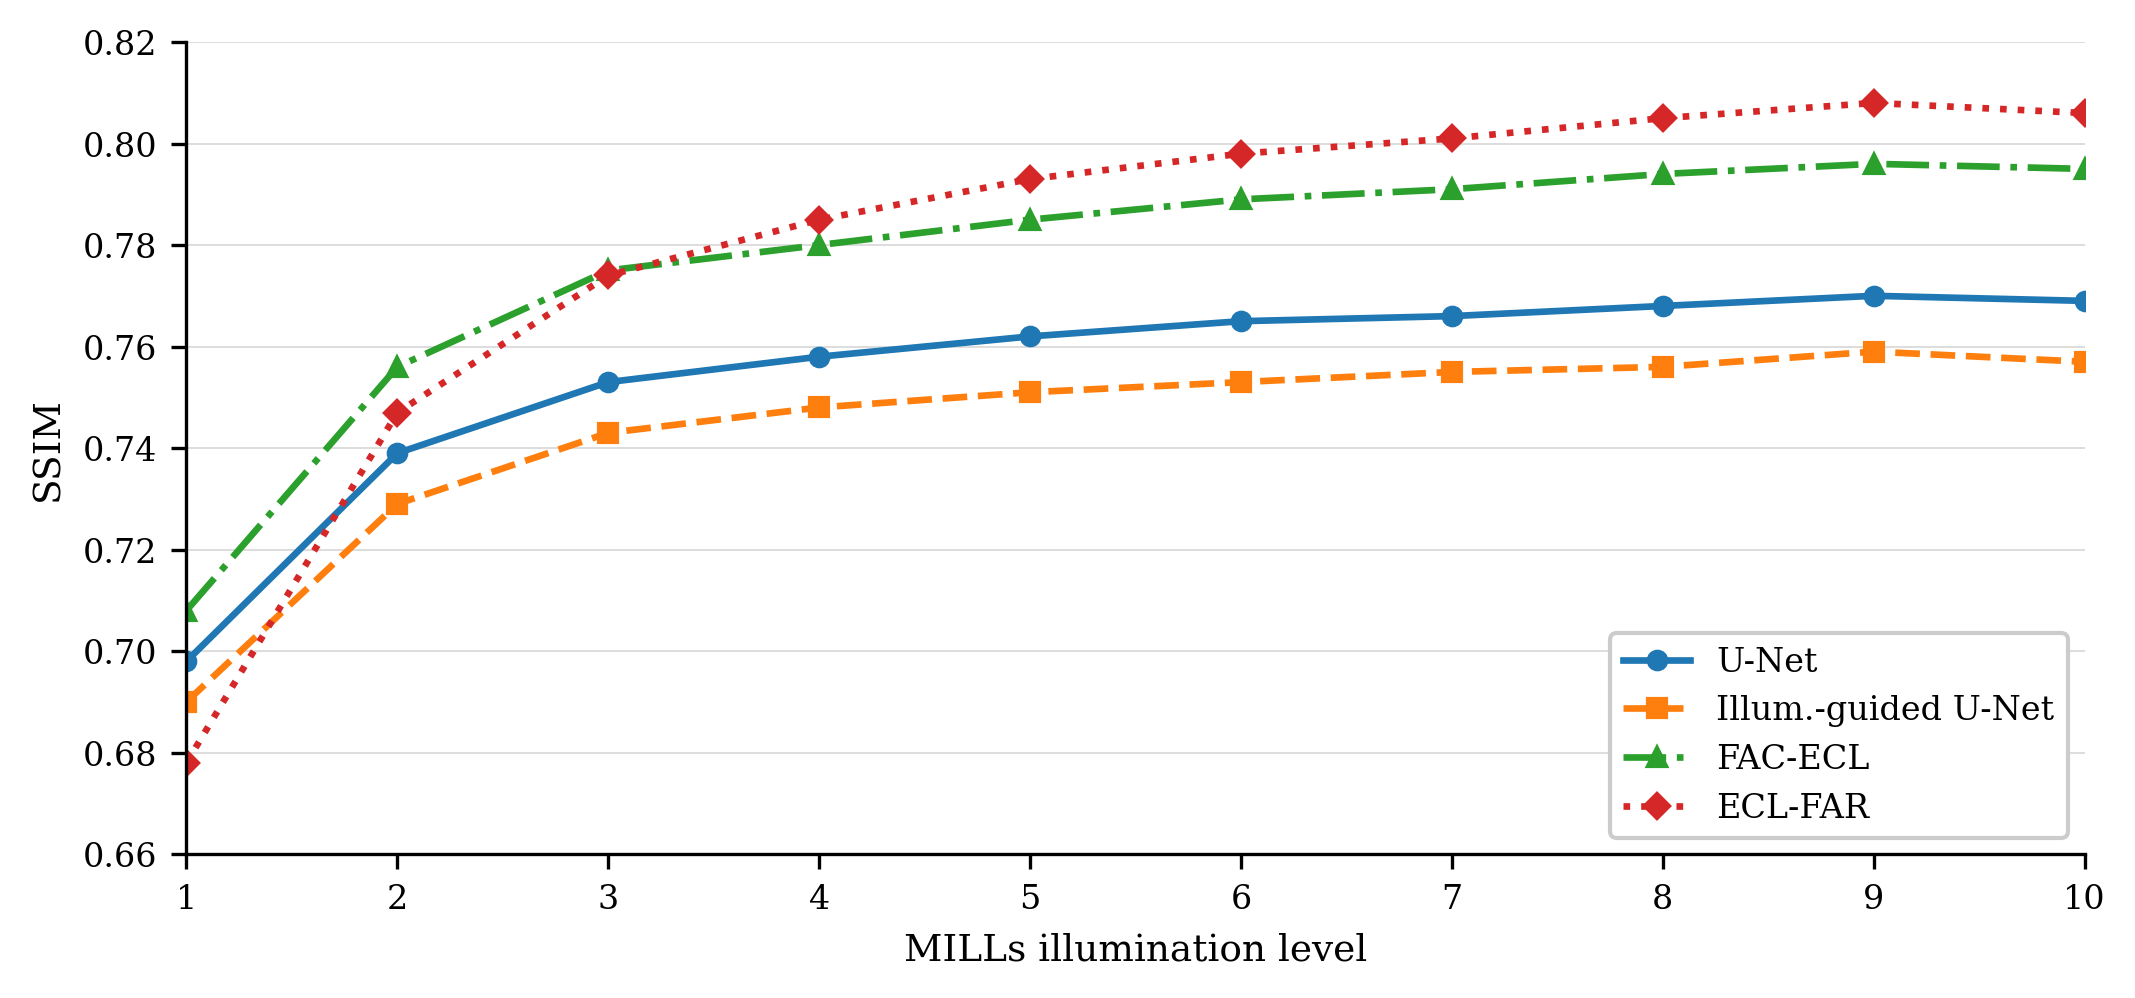
\includegraphics[width=\textwidth]{fig/mills_ssim_by_illumination/mills_ssim_by_illumination.png}
	\caption{MILLs illumination-level SSIM trend for the selected configuration of each model family. Each point reports the mean SSIM across three seeds at the corresponding illumination level. Higher values indicate better structural similarity.}
	\label{fig:mills_ssim_by_illumination}
\end{figure*}

The baseline U-Net already shows this behavior. Its SSIM grows from 0.698 at level 1 to about 0.770 at level 9, while the dark-pixel ratio decreases from 3.3\% to about 0.3\%. The illumination-guided U-Net reduces residual darkness, but this does not improve the paired reconstruction. Its level-1 dark-pixel ratio is lower than the baseline, but its SSIM is also lower. This means that making the image brighter is not the same as making it closer to the target. The model can remove darkness while still introducing wrong color, wrong contrast, or structural errors.

FAC-ECL improves the MILLs trend. Its SSIM rises from 0.708 at level 1 to 0.796 at level 9, and it obtains the best global MAE on MILLs among the four families. This suggests that frequency-aware supervision helps the model separate broad illumination correction from local detail preservation. ECL-FAR pushes the structural result slightly further, reaching 0.808 SSIM at level 9, which is the best illumination-level SSIM observed in the report. However, ECL-FAR is weaker at level 1 and has a higher RGB imbalance across MILLs levels. This means that its refinement mechanism is most useful when the first enhancement already contains enough reliable structure. When the input is extremely dark, the instability map can indicate uncertainty, but it cannot recover details that are almost absent.

The MILLs analysis gives a general lesson. A good low-light model should not only increase exposure. It must adapt the correction to the amount of information present in the input. FAC-ECL and ECL-FAR do this better than the first two families, especially from medium to high illumination levels. The hardest case remains the darkest level, where all models are limited by the lack of reliable visual signal. This pattern also explains why average dataset-level scores should be read together with illumination-level results: global improvements can hide different behavior at darkest inputs.

\analysispar{Patterns across ExDark categories}
The category-level ExDark results show stable patterns across the four families. The best NIQE category is always motorbike, while the worst NIQE category is always boat. For BRISQUE, cup is consistently the worst category, while the best category is usually bicycle, except for the baseline U-Net, where dog obtains the best BRISQUE.

These patterns should not be interpreted as purely semantic effects. The model is not necessarily better because the object is a motorbike, or worse because the object is a boat or a cup. A more plausible explanation is that each category is associated with recurring visual conditions. Motorbike and bicycle images often contain strong edges, visible object contours, and local contrast, which can make the enhanced images closer to natural-image statistics. Boat images often contain large dark backgrounds, water, sky, or low-contrast regions, where the input signal is weak and the enhancement can become either noisy or over-smoothed. Cup and bottle images often contain small indoor objects, strong shadows, and background clutter. These scenes can remain under-exposed and can also show color shifts after enhancement.

The diagnostic metrics support this interpretation. Bottle and cup often have among the lowest mean luminance values and among the highest dark-pixel ratios. This means that these categories remain difficult because many pixels are still too dark after enhancement. Car images often have the highest clipping ratio. This is expected because cars frequently contain headlights, reflective surfaces, or small bright highlights; when the model brightens the whole scene, those regions can become saturated. RGB imbalance is also high in several object categories, especially bottle, cup, bus, bicycle, and car depending on the family. This indicates that color cast is a recurring cross-dataset failure on ExDark.

Therefore, the ExDark category analysis suggests that the main difficulty is not the object label itself, but the visual conditions correlated with that label: amount of usable signal, local light sources, reflective materials, background darkness, and color distribution. This is important for cross-dataset generalization, because it shows that a model trained on LOL-v2 Real does not fail randomly. It fails more often when the test image combines weak input signal, strong local highlights, and unfamiliar color statistics.

\subsection{Qualitative Inter-Family Comparison}

Figure~\ref{fig:inter_family_random_panel} compares the selected configurations of all four families on the same visual examples. The final panel was built by combining two independent inter-family export runs. Since each run randomly selects one test image from each evaluation dataset, the combined panel contains two random examples for each dataset. For paired datasets, the corresponding target image is shown in the last column. For ExDark, the target column is marked as not available because the dataset is unpaired. Each row therefore allows a direct comparison between the input, the four enhanced outputs, and the target when it exists. Because the examples are randomly sampled rather than selected for a failure mode, the panel is not intended to favor any family. Instead, it provides a visual complement to the dataset-level results, showing how the selected models behave on identical content.

\begin{figure*}[p]
	\centering
	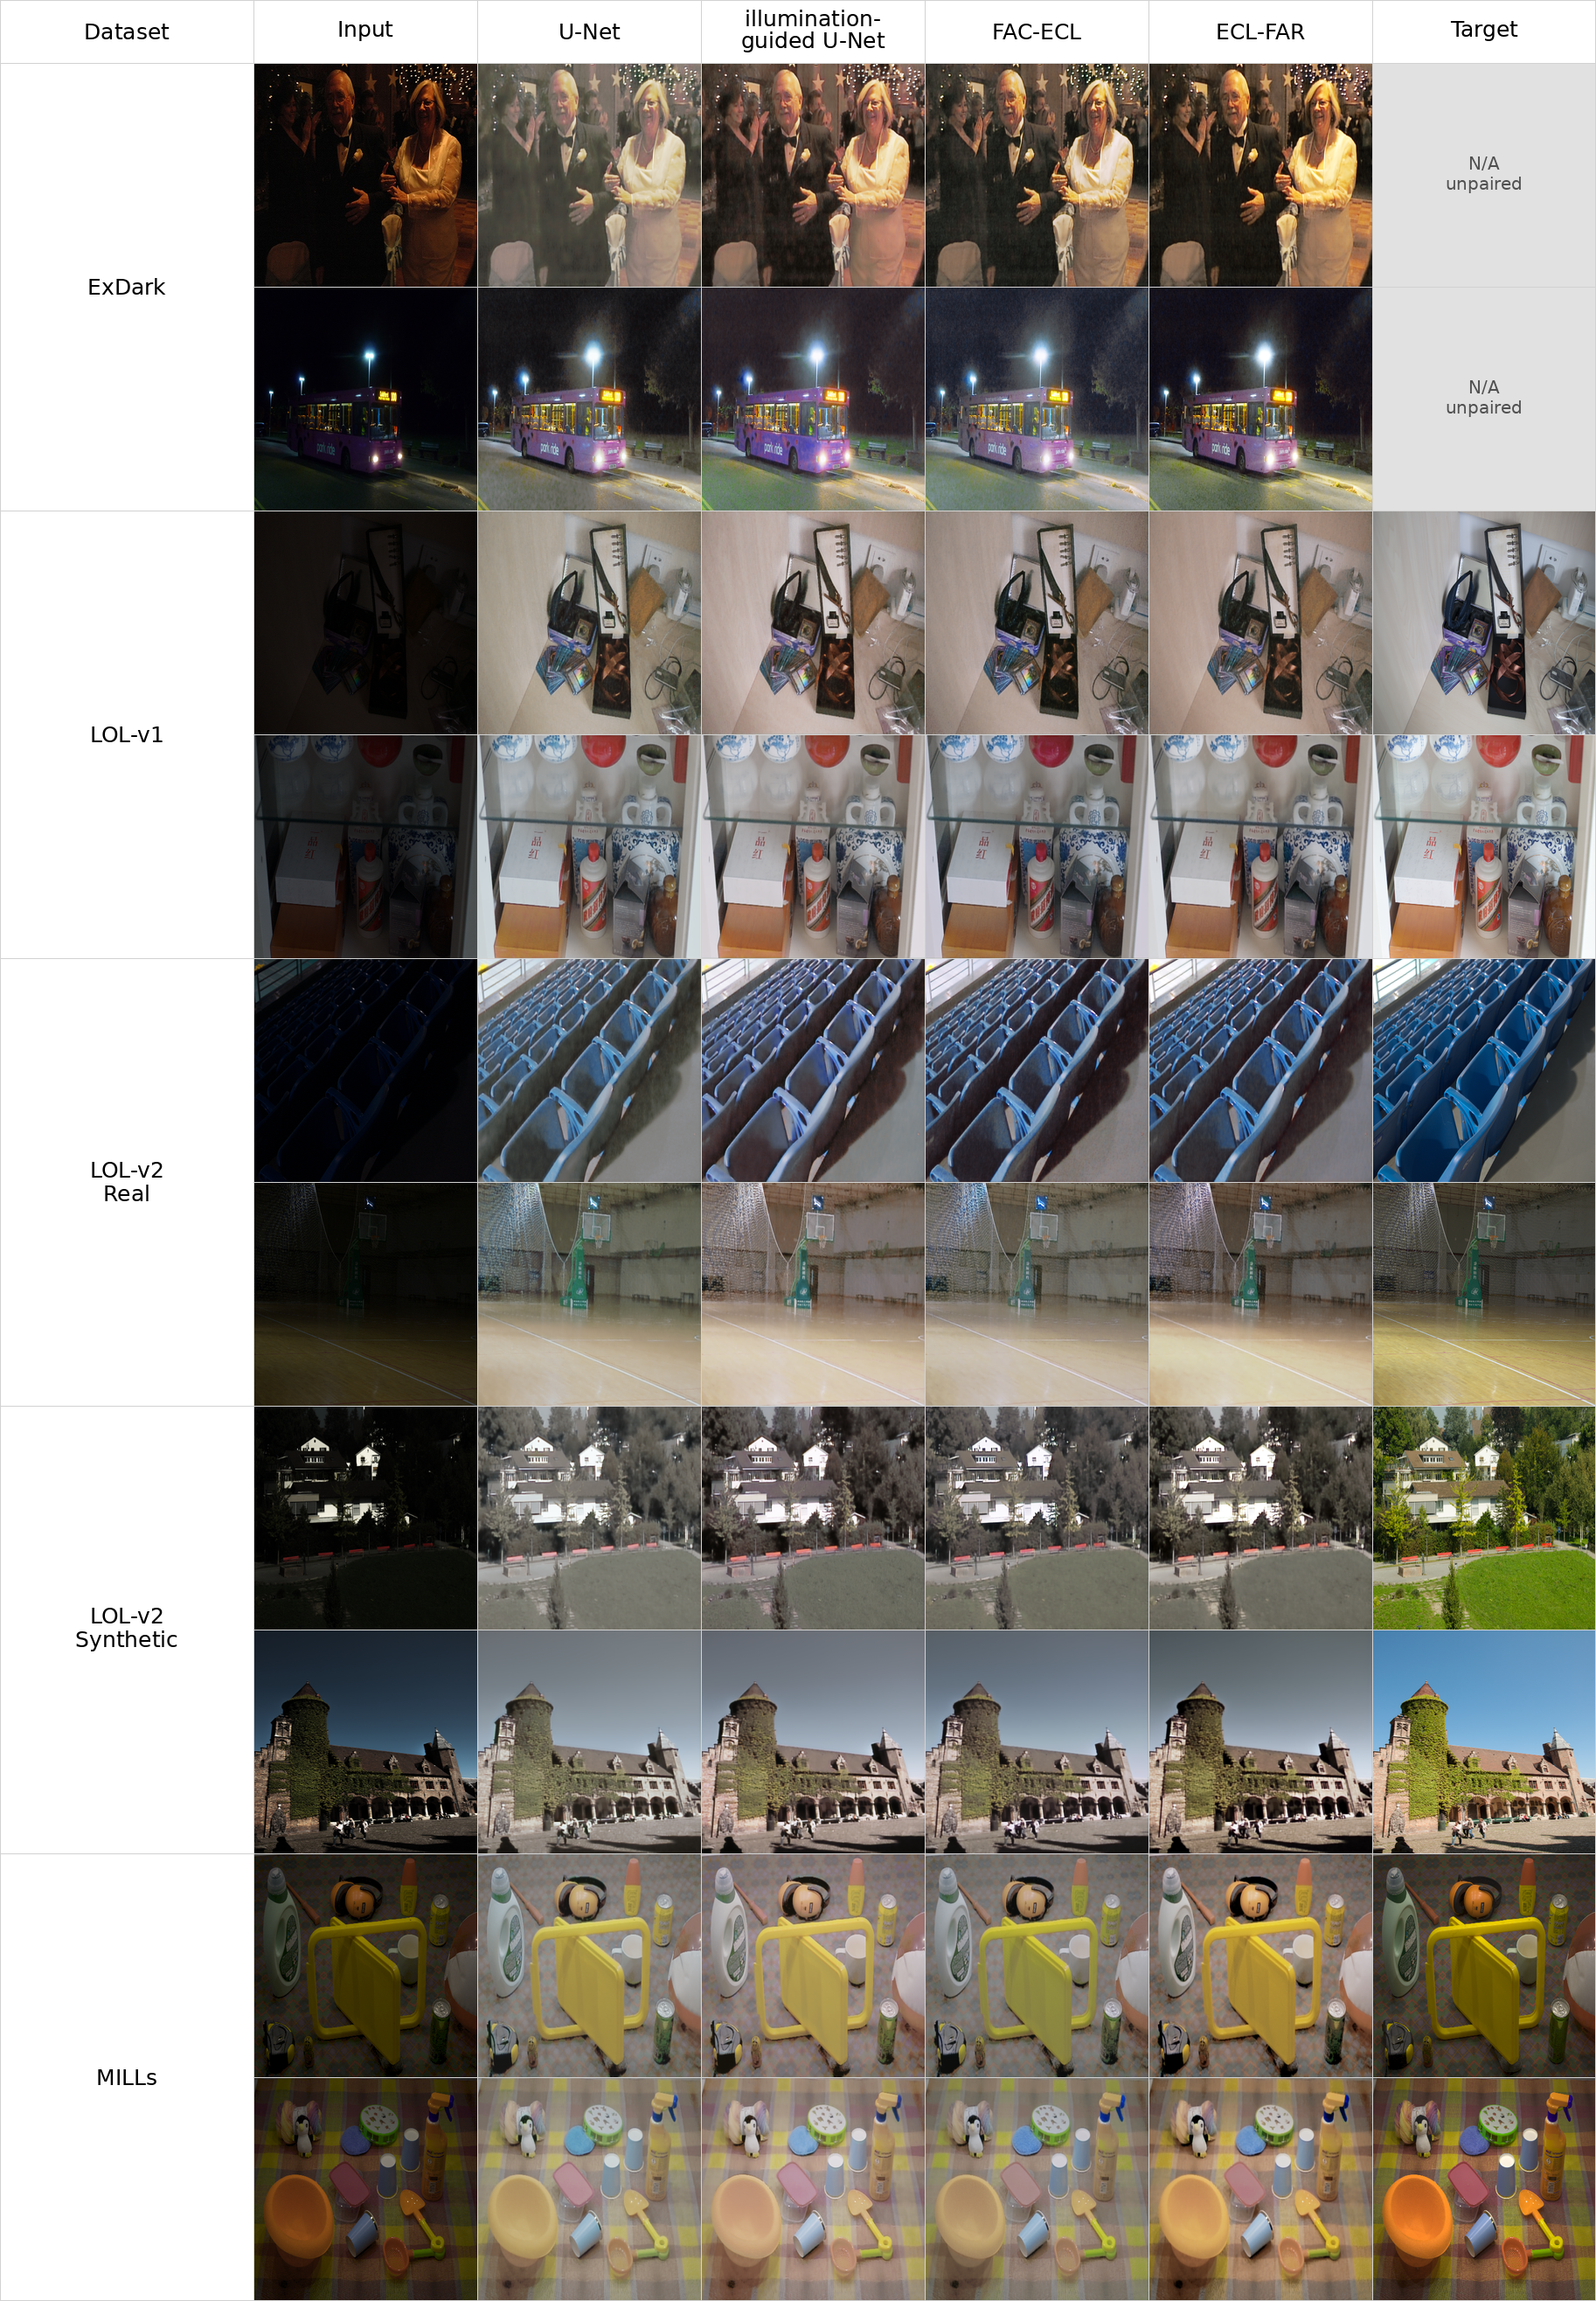
\includegraphics[
	height=\dimexpr\textheight-4\baselineskip\relax,
	keepaspectratio
	]{fig/inter_family_random_panel/inter_family_random_panel.png}
	\caption{Inter-family qualitative comparison on two random test examples for each dataset. Each individual export run selects one random test sample per dataset; the figure combines two independent runs to show two examples for each dataset. Rows are ordered as LOL-v2 Real, LOL-v2 Synthetic, MILLs, ExDark, and LOL-v1 (overlap). Each row contains the low-light input, the enhanced output produced by each selected model family, and the target image when available.}
	\label{fig:inter_family_random_panel}
\end{figure*}

\analysispar{LOL-v2 Real examples}
The two LOL-v2 Real examples show the in-domain behavior. Since the models are trained on LOL-v2 Real, all outputs are plausible. However, the row with the blue seats highlights an important difference. The baseline U-Net tends to produce a flatter and more gray result. The illumination-guided U-Net and FAC-ECL improve the exposure, but the output can still look slightly washed out. ECL-FAR better preserves the blue color of the seats and remains closer to the target appearance. In the court example, the final families also produce a more controlled enhancement than the first two families. This supports the idea that the later variants do not simply brighten the image, but better control structure and color in many in-domain cases.

\analysispar{LOL-v2 Synthetic examples}
The two LOL-v2 Synthetic examples are the clearest evidence that synthetic low-light degradation is problematic for models trained on real low-light data. In the house example, the target has natural green vegetation and a bright outdoor appearance. All model outputs remain gray, desaturated, and far from the target. In the building example, the target has a blue sky, green vegetation, and a much more natural color balance. The enhanced outputs improve visibility, but none of them fully recovers the target color distribution. ECL-FAR sometimes preserves slightly more color than the other families, but the gap with the target remains large. These examples explain why the synthetic dataset is unreliable in this protocol: the model has learned from real under-exposed images, but the synthetic inputs follow a different degradation process. The result is that the model can brighten the image without learning the specific inverse transformation required by the synthetic target.

\analysispar{MILLs examples}
The two MILLs examples are useful for judging color preservation. Both inputs are dark but contain many colored objects. The baseline U-Net produces pale, desaturated outputs. The illumination-guided U-Net improves visibility, but some colors remain unstable. FAC-ECL is more balanced and closer to the paired target in reconstruction metrics. ECL-FAR gives the most convincing color preservation. In the first row, the yellow object is more recognizable and less washed out; in the second, the orange bowl and colored toys retain stronger saturation, although the output is not perfect. This agrees with the observation that ECL-FAR can preserve color better locally. However, its RGB imbalance on MILLs shows that color preservation is not fully solved: visually good examples do not imply consistent chromatic accuracy across the dataset.

\analysispar{ExDark examples}
The two ExDark examples show the behavior on real unpaired dark scenes. In the first row, the input contains people in a very dark environment. The baseline U-Net and the illumination-guided U-Net increase visibility, but the dark clothing becomes gray and dirty, and the image contains a visible haze. FAC-ECL improves the overall balance, but the output still looks slightly veiled. ECL-FAR gives the cleanest visual result in this row: the black jacket of the man remains less contaminated by gray noise, and the colors of the people are better preserved. In the second ExDark row, the bus is surrounded by a very dark sky. Again, the simpler families brighten the scene but leave a dirtier dark background. ECL-FAR preserves the dark sky more cleanly and keeps the bus color more stable. These comparisons do not establish target fidelity, because ExDark is unpaired, but they help reveal visually disturbing artifacts in severely dark real-world scenes. These two examples show the qualitative strength of ECL-FAR on some real dark scenes, even though the global ExDark diagnostics show that it can also be conservative and leave more dark pixels on average.

\analysispar{LOL-v1 (overlap) examples}
The two LOL-v1 (overlap) examples are descriptive controls from the overlapping LOL-v1/LOL-v2 Real image pool. All models produce reasonable outputs, and the differences are smaller than on the other datasets. The baseline U-Net already recovers most of the scene. The illumination-guided U-Net sometimes brightens the image slightly more, but this does not always make it closer to the target. FAC-ECL and ECL-FAR usually give the most balanced results, with good visibility and fewer obvious artifacts. Their role is to show how the selected models behave on shared content under the same paired setting. Because the underlying inputs overlap with the LOL-v2 Real pool, their apparent agreement with the targets is more informative about within-pool behavior than robustness to new acquisition conditions. These examples are reported for descriptive transparency only and are not used as evidence of independent cross-dataset transfer or model ranking.

\analysispar{Summary}
Overall, the qualitative panel shows a clear progression. The baseline U-Net is a strong and simple reference, but it often produces gray, hazy, or desaturated outputs under distribution shift. The illumination-guided U-Net makes the local brightness information explicit, but this mainly helps exposure and does not reliably improve target fidelity. FAC-ECL is the most important improvement from the training-objective point of view: it improves paired cross-dataset reconstruction, especially on MILLs, by separating low-frequency illumination behavior from high-frequency detail behavior and by encouraging exposure consistency. ECL-FAR adds a refinement mechanism based on photometric instability. In the selected visual examples, it often preserves colors more effectively and keeps dark regions cleaner, especially on ExDark and MILLs. This visual advantage is coherent with its strongest structural result on MILLs, but should not override its weaker behavior on LOL-v2 Synthetic or its mixed ExDark diagnostics. However, this qualitative advantage remains example-dependent and should be interpreted together with the dataset-level diagnostic results.

\subsection{Final Inter-Family Summary}

Considering the full set of evidence, the best family depends on the criterion used. If the main criterion is paired reconstruction on shifted paired datasets, FAC-ECL and ECL-FAR are the strongest families. FAC-ECL is the safest quantitative improvement because it improves MILLs clearly and remains balanced across most metrics. ECL-FAR obtains the best SSIM on MILLs and gives the most convincing qualitative color preservation in the final comparison panel. For this reason, ECL-FAR can be considered a strong family when structural performance on MILLs and qualitative appearance are prioritized. This distinction matters because reconstruction metrics and visual plausibility capture complementary aspects of low-light enhancement.

This conclusion must be stated with a caveat. ECL-FAR is not a complete solution. On LOL-v2 Synthetic, it is weaker than the other families, which confirms that synthetic degradation remains a difficult and partly misleading distribution shift. On ExDark, it obtains the best NIQE but the worst BRISQUE, and its diagnostic metrics show more residual darkness and stronger RGB imbalance. Therefore, ECL-FAR is best read as a promising refinement-based extension rather than as a universally dominant model. This point is especially relevant because ECL-FAR is an original idea introduced in this project and tested as a first implementation. It was not exhaustively optimized in all its components, such as the instability map, the refinement module, the residual scale, or the perturbation policy. Accordingly, its current results should be interpreted as evidence of feasibility rather than as a final architecture-level optimum. The fact that it is already competitive with FAC-ECL, and in some cases stronger, suggests that the refinement idea has practical value and deserves a deeper dedicated study. This is particularly clear in the qualitative comparison panel, where ECL-FAR is often the most convincing family in the selected examples.

The most important insight of the whole inter-family analysis is that low-light enhancement cannot be reduced to brightness increase. The illumination-guided U-Net demonstrates this clearly: it can reduce dark pixels, but it does not necessarily improve SSIM, PSNR, MAE, or color stability. The better families are those that constrain how the enhancement is performed. FAC-ECL constrains low-frequency illumination and high-frequency detail separately. ECL-FAR uses photometric sensitivity to decide where local refinement may be useful. These ideas improve cross-dataset behavior because they address the real failure modes of low-light enhancement. In particular, instability-guided refinement can complement conventional reconstruction objectives when illumination conditions change.

The final conclusion is therefore that ECL-FAR is a promising model family, especially from a qualitative and structural point of view on MILLs.